\documentclass{standalone}
\usepackage{tikz}
\usetikzlibrary{patterns, positioning}


\begin{document}
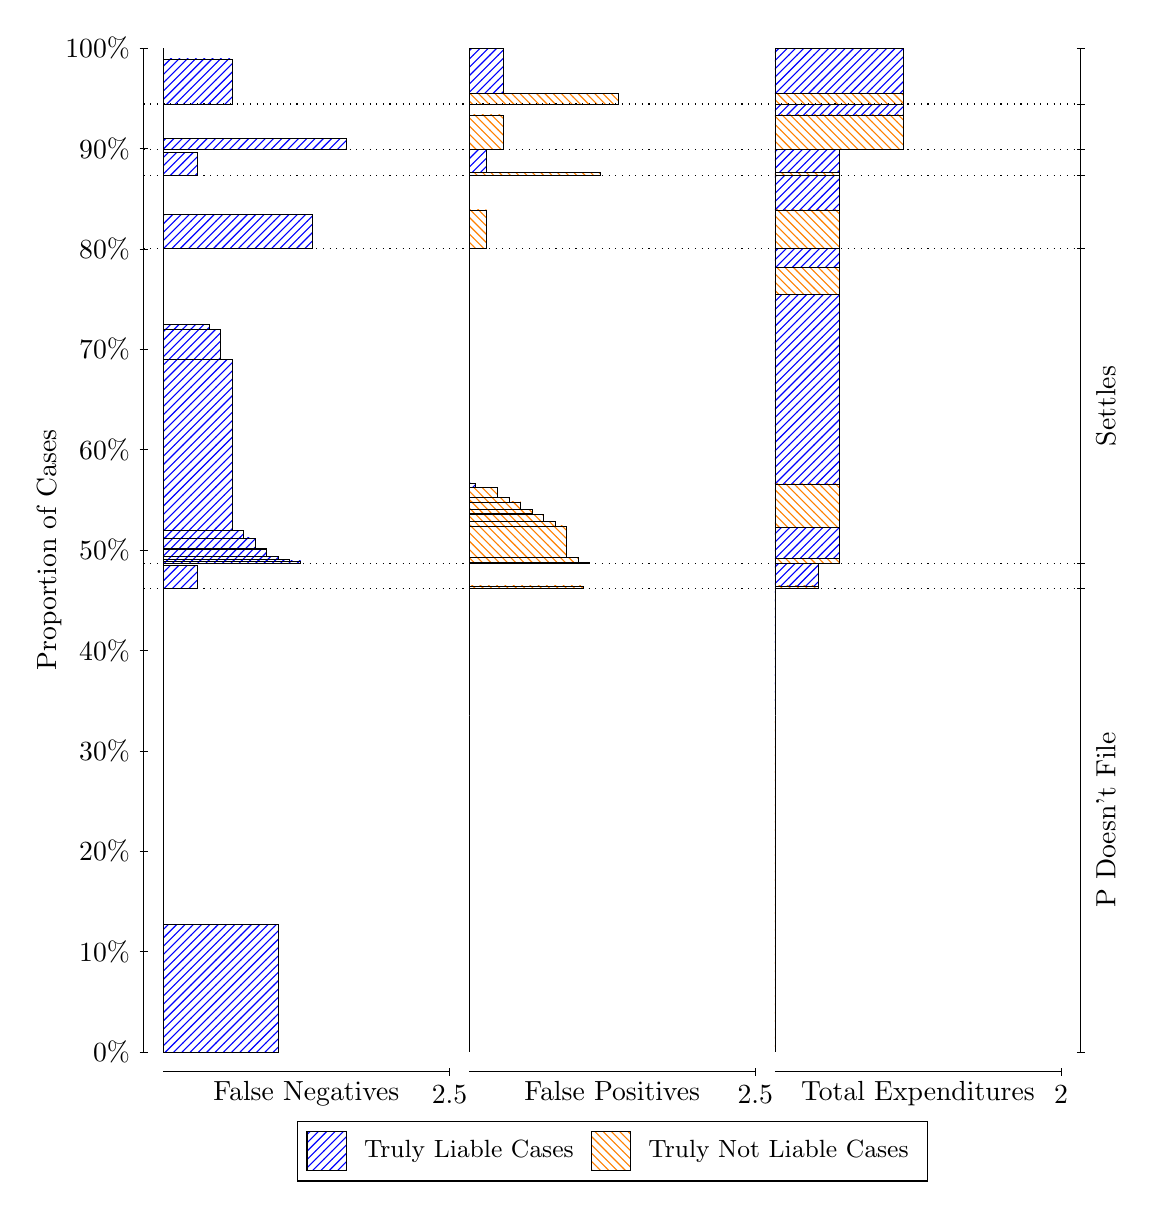
\begin{tikzpicture}
\draw[black, very thin] (1.5,1.75) -- (1.5,14.5);
\node[rotate=90, text=black, anchor=center] at (0.3, 8.125) {Proportion of Cases};
\draw[black, very thin] (1.45,1.75) -- (1.55,1.75);
\node[text=black, anchor=east] at (1.45, 1.75) {0\%};
\draw[black, very thin] (1.45,3.025) -- (1.55,3.025);
\node[text=black, anchor=east] at (1.45, 3.025) {10\%};
\draw[black, very thin] (1.45,4.3) -- (1.55,4.3);
\node[text=black, anchor=east] at (1.45, 4.3) {20\%};
\draw[black, very thin] (1.45,5.575) -- (1.55,5.575);
\node[text=black, anchor=east] at (1.45, 5.575) {30\%};
\draw[black, very thin] (1.45,6.85) -- (1.55,6.85);
\node[text=black, anchor=east] at (1.45, 6.85) {40\%};
\draw[black, very thin] (1.45,8.125) -- (1.55,8.125);
\node[text=black, anchor=east] at (1.45, 8.125) {50\%};
\draw[black, very thin] (1.45,9.4) -- (1.55,9.4);
\node[text=black, anchor=east] at (1.45, 9.4) {60\%};
\draw[black, very thin] (1.45,10.675) -- (1.55,10.675);
\node[text=black, anchor=east] at (1.45, 10.675) {70\%};
\draw[black, very thin] (1.45,11.95) -- (1.55,11.95);
\node[text=black, anchor=east] at (1.45, 11.95) {80\%};
\draw[black, very thin] (1.45,13.225) -- (1.55,13.225);
\node[text=black, anchor=east] at (1.45, 13.225) {90\%};
\draw[black, very thin] (1.45,14.5) -- (1.55,14.5);
\node[text=black, anchor=east] at (1.45, 14.5) {100\%};

\draw[black, very thin] (13.4,1.75) -- (13.4,14.5);
\draw[black, very thin] (13.35,1.75) -- (13.45,1.75);
\node[anchor=west] at (13.35, 1.75) {};
\draw[black, very thin] (13.35,7.641) -- (13.45,7.641);
\node[anchor=west] at (13.35, 7.641) {};
\draw[black, very thin] (13.35,7.9564) -- (13.45,7.9564);
\node[anchor=west] at (13.35, 7.9564) {};
\draw[black, very thin] (13.35,11.952) -- (13.45,11.952);
\node[anchor=west] at (13.35, 11.952) {};
\draw[black, very thin] (13.35,12.879) -- (13.45,12.879);
\node[anchor=west] at (13.35, 12.879) {};
\draw[black, very thin] (13.35,13.214) -- (13.45,13.214);
\node[anchor=west] at (13.35, 13.214) {};
\draw[black, very thin] (13.35,13.789) -- (13.45,13.789);
\node[anchor=west] at (13.35, 13.789) {};
\draw[black, very thin] (13.35,14.5) -- (13.45,14.5);
\node[anchor=west] at (13.35, 14.5) {};

\draw[black, very thin, pattern color=blue, pattern=north east lines] (1.75,1.75) rectangle (3.2033,3.3658);
\draw[black, very thin, pattern color=orange, pattern=north west lines] (1.75,3.3658) rectangle (1.75,7.641);
\draw[black, very thin, pattern color=blue, pattern=north east lines] (1.75,7.641) rectangle (2.186,7.9291);
\draw[black, very thin, pattern color=orange, pattern=north west lines] (1.75,7.9291) rectangle (1.75,7.9564);
\draw[black, very thin, pattern color=blue, pattern=north east lines] (1.75,7.9564) rectangle (3.494,7.9869);
\draw[black, very thin, pattern color=blue, pattern=north east lines] (1.75,7.9869) rectangle (3.3487,8.0092);
\draw[black, very thin, pattern color=blue, pattern=north east lines] (1.75,8.0092) rectangle (3.2033,8.0474);
\draw[black, very thin, pattern color=blue, pattern=north east lines] (1.75,8.0474) rectangle (3.058,8.136);
\draw[black, very thin, pattern color=blue, pattern=north east lines] (1.75,8.136) rectangle (3.058,8.1466);
\draw[black, very thin, pattern color=blue, pattern=north east lines] (1.75,8.1466) rectangle (2.9127,8.2802);
\draw[black, very thin, pattern color=blue, pattern=north east lines] (1.75,8.2802) rectangle (2.7673,8.3783);
\draw[black, very thin, pattern color=blue, pattern=north east lines] (1.75,8.3783) rectangle (2.622,10.541);
\draw[black, very thin, pattern color=blue, pattern=north east lines] (1.75,10.541) rectangle (2.4767,10.931);
\draw[black, very thin, pattern color=blue, pattern=north east lines] (1.75,10.931) rectangle (2.3313,10.989);
\draw[black, very thin, pattern color=orange, pattern=north west lines] (1.75,10.989) rectangle (1.75,11.952);
\draw[black, very thin, pattern color=blue, pattern=north east lines] (1.75,11.952) rectangle (3.6393,12.386);
\draw[black, very thin, pattern color=orange, pattern=north west lines] (1.75,12.386) rectangle (1.75,12.879);
\draw[black, very thin, pattern color=blue, pattern=north east lines] (1.75,12.879) rectangle (2.186,13.174);
\draw[black, very thin, pattern color=orange, pattern=north west lines] (1.75,13.174) rectangle (1.75,13.214);
\draw[black, very thin, pattern color=blue, pattern=north east lines] (1.75,13.214) rectangle (4.0753,13.352);
\draw[black, very thin, pattern color=orange, pattern=north west lines] (1.75,13.352) rectangle (1.75,13.789);
\draw[black, very thin, pattern color=blue, pattern=north east lines] (1.75,13.789) rectangle (2.622,14.362);
\draw[black, very thin, pattern color=orange, pattern=north west lines] (1.75,14.362) rectangle (1.75,14.5);
\draw[black, very thin, pattern color=orange, pattern=north west lines] (5.6333,1.75) rectangle (5.6333,6.0252);
\draw[black, very thin, pattern color=blue, pattern=north east lines] (5.6333,6.0252) rectangle (5.6333,7.641);
\draw[black, very thin, pattern color=orange, pattern=north west lines] (5.6333,7.641) rectangle (7.0867,7.6683);
\draw[black, very thin, pattern color=blue, pattern=north east lines] (5.6333,7.6683) rectangle (5.6333,7.9564);
\draw[black, very thin, pattern color=orange, pattern=north west lines] (5.6333,7.9564) rectangle (7.1593,7.9695);
\draw[black, very thin, pattern color=orange, pattern=north west lines] (5.6333,7.9695) rectangle (7.014,8.035);
\draw[black, very thin, pattern color=orange, pattern=north west lines] (5.6333,8.035) rectangle (6.8687,8.4326);
\draw[black, very thin, pattern color=orange, pattern=north west lines] (5.6333,8.4326) rectangle (6.7233,8.4912);
\draw[black, very thin, pattern color=orange, pattern=north west lines] (5.6333,8.4912) rectangle (6.578,8.5805);
\draw[black, very thin, pattern color=orange, pattern=north west lines] (5.6333,8.5805) rectangle (6.4327,8.5889);
\draw[black, very thin, pattern color=orange, pattern=north west lines] (5.6333,8.5889) rectangle (6.4327,8.6429);
\draw[black, very thin, pattern color=orange, pattern=north west lines] (5.6333,8.6429) rectangle (6.2873,8.7368);
\draw[black, very thin, pattern color=orange, pattern=north west lines] (5.6333,8.7368) rectangle (6.142,8.7952);
\draw[black, very thin, pattern color=orange, pattern=north west lines] (5.6333,8.7952) rectangle (5.9967,8.9199);
\draw[black, very thin, pattern color=blue, pattern=north east lines] (5.6333,8.9199) rectangle (5.706,8.9779);
\draw[black, very thin, pattern color=blue, pattern=north east lines] (5.6333,8.9779) rectangle (5.6333,11.952);
\draw[black, very thin, pattern color=orange, pattern=north west lines] (5.6333,11.952) rectangle (5.8513,12.445);
\draw[black, very thin, pattern color=blue, pattern=north east lines] (5.6333,12.445) rectangle (5.6333,12.879);
\draw[black, very thin, pattern color=orange, pattern=north west lines] (5.6333,12.879) rectangle (7.3047,12.919);
\draw[black, very thin, pattern color=blue, pattern=north east lines] (5.6333,12.919) rectangle (5.8513,13.214);
\draw[black, very thin, pattern color=orange, pattern=north west lines] (5.6333,13.214) rectangle (6.0693,13.652);
\draw[black, very thin, pattern color=blue, pattern=north east lines] (5.6333,13.652) rectangle (5.6333,13.789);
\draw[black, very thin, pattern color=orange, pattern=north west lines] (5.6333,13.789) rectangle (7.5227,13.928);
\draw[black, very thin, pattern color=blue, pattern=north east lines] (5.6333,13.928) rectangle (6.0693,14.5);
\draw[black, very thin, pattern color=orange, pattern=north west lines] (9.5167,1.75) rectangle (9.5167,6.0252);
\draw[black, very thin, pattern color=blue, pattern=north east lines] (9.5167,6.0252) rectangle (9.5167,7.641);
\draw[black, very thin, pattern color=orange, pattern=north west lines] (9.5167,7.641) rectangle (10.062,7.6683);
\draw[black, very thin, pattern color=blue, pattern=north east lines] (9.5167,7.6683) rectangle (10.062,7.9564);
\draw[black, very thin, pattern color=orange, pattern=north west lines] (9.5167,7.9564) rectangle (10.334,8.0219);
\draw[black, very thin, pattern color=blue, pattern=north east lines] (9.5167,8.0219) rectangle (10.334,8.4118);
\draw[black, very thin, pattern color=orange, pattern=north west lines] (9.5167,8.4118) rectangle (10.334,8.9657);
\draw[black, very thin, pattern color=blue, pattern=north east lines] (9.5167,8.9657) rectangle (10.334,11.37);
\draw[black, very thin, pattern color=orange, pattern=north west lines] (9.5167,11.37) rectangle (10.334,11.714);
\draw[black, very thin, pattern color=blue, pattern=north east lines] (9.5167,11.714) rectangle (10.334,11.952);
\draw[black, very thin, pattern color=orange, pattern=north west lines] (9.5167,11.952) rectangle (10.334,12.445);
\draw[black, very thin, pattern color=blue, pattern=north east lines] (9.5167,12.445) rectangle (10.334,12.879);
\draw[black, very thin, pattern color=orange, pattern=north west lines] (9.5167,12.879) rectangle (10.334,12.919);
\draw[black, very thin, pattern color=blue, pattern=north east lines] (9.5167,12.919) rectangle (10.334,13.214);
\draw[black, very thin, pattern color=orange, pattern=north west lines] (9.5167,13.214) rectangle (11.152,13.652);
\draw[black, very thin, pattern color=blue, pattern=north east lines] (9.5167,13.652) rectangle (11.152,13.789);
\draw[black, very thin, pattern color=orange, pattern=north west lines] (9.5167,13.789) rectangle (11.152,13.928);
\draw[black, very thin, pattern color=blue, pattern=north east lines] (9.5167,13.928) rectangle (11.152,14.5);
\draw[black, dotted] (1.5,7.641) -- (13.4,7.641);
\draw[black, dotted] (1.5,7.9564) -- (13.4,7.9564);
\draw[black, dotted] (1.5,11.952) -- (13.4,11.952);
\draw[black, dotted] (1.5,12.879) -- (13.4,12.879);
\draw[black, dotted] (1.5,13.214) -- (13.4,13.214);
\draw[black, dotted] (1.5,13.789) -- (13.4,13.789);
\draw[black, very thin] (1.75,1.5) -- (5.3833,1.5);
\node[text=black, anchor=north] at (3.5667, 1.5) {False Negatives};
\draw[black, very thin] (5.3833,1.45) -- (5.3833,1.55);
\node[text=black, anchor=north] at (5.3833, 1.45) {2.5};

\draw[black, very thin] (5.6333,1.5) -- (9.2667,1.5);
\node[text=black, anchor=north] at (7.45, 1.5) {False Positives};
\draw[black, very thin] (9.2667,1.45) -- (9.2667,1.55);
\node[text=black, anchor=north] at (9.2667, 1.45) {2.5};

\draw[black, very thin] (9.5167,1.5) -- (13.15,1.5);
\node[text=black, anchor=north] at (11.333, 1.5) {Total Expenditures};
\draw[black, very thin] (13.15,1.45) -- (13.15,1.55);
\node[text=black, anchor=north] at (13.15, 1.45) {2};

\node[text=black, centered, rotate=90] at (13.72, 4.6955) {P Doesn't File};

\node[text=black, centered, rotate=90] at (13.72, 9.9542) {Settles};





\draw (7.449999999999999,1.5) node[draw=none] (baseCoordinate) {};
\begin{scope}[align=center]
        \matrix[scale=0.5, draw=black, below=0.5cm of baseCoordinate, nodes={draw}, column sep=0.1cm]{
            \node[rectangle, draw, minimum width=0.5cm, minimum height=0.5cm, pattern color=blue, pattern=north east lines] {}; &
            \node[draw=none, font=\small, text=black] (B) {Truly Liable Cases}; &
            \node[rectangle, draw, minimum width=0.5cm, minimum height=0.5cm, pattern color=orange, pattern=north west lines] {}; &
            \node[draw=none, font=\small, text=black] (B) {Truly Not Liable Cases}; \\
            };
\end{scope}

\end{tikzpicture}
\end{document}